\subsection{拓扑群的右一致结构与左一致结构}

在拓扑群 G 中，我们可以察觉到按下述方式定义“充分近的点”这个概念、从而定义一个一致结构的可能性：若 x 与 y 是 G 的任意两点，我们对这两点施加把其中之一（比如说 x）送到单位元 e 的平移；x 与 y 的“接近程度”这时在某种意义上由 y 被送入的 e 的邻域 V 来衡量。这个平移——它在于把 x 与 y 都乘以 \(x^{-1}\)——可以在右边或在左边进行，而我们将看到，在这两种情形我们都确实得到 G 上的一个与 G 的拓扑相容的一致结构。取平移在右边进行的情形；于是对 e 的每个邻域 V 对应有集 \(V_{d}\)，即偶 \((x, y) \in \mathbf{G} \times \mathbf{G}\)（满足 \(yx^{-1} \in V\) 的）组成的集。设 \(G_{d}\) 是诸集 \(V_{d}\) 的族，其中 V 跑遍 e 的邻域滤子 B。则 \(G_{d}\) 是一个基本一致邻域系（第二章 § 1 第 1 目）。因为由于 \(e \in V\)，对角线 \(\Delta\)（\(G \times G\) 的）含于 \(V_{d}\)（对每个 \(V \in B\)），于是 \(G_{d}\) 是一个滤子基且满足公理 \((\mathrm{U}_{\mathrm{I}}^{\prime})\)；由于关系 \(yx^{-1} \in V\) 与 \(xy^{-1} \in V^{-1}\) 等价，我们有 \(\mathbf{V}_{d}^{-1} = (\mathbf{V}^{-1})_{d}\)。

于是 \(\mathbf{V}_{d}^{-1}\in \mathfrak{G}_d\)（由 \((\mathrm{GV}_{\mathrm{II}})\)），从而 \((\mathrm{U}_{\mathrm{II}}^{\prime})\) 满足；最后，关系 \(zx^{-1}\in \mathrm{V}\) 与 \(yz^{-1}\in \mathrm{V}\) 蕴含 \(yx^{-1}\in \mathrm{V.V}\)；于是 \(\mathbf{V}_d\circ \mathbf{V}_d\) 含于 \((\mathrm{V.V})_d\)，而 \((\mathrm{GV}_{\mathrm{I}})\) 表明 \(\mathfrak{G}_d\) 满足 \((\mathrm{U}_{\mathrm{III}}^{\prime})\)。

由 \(\mathfrak{G}_d\) 定义的一致结构与 \(\mathbf{G}\) 的拓扑相容，因为关系 \(y \in \mathrm{V}_d(x)\) 与 \(y \in \mathrm{V}.x\) 依定义等价；换言之，\(\mathrm{V}_d(x) = \mathrm{V}.x\)。

当平移在左边进行时，论证是类似的，因此我们可以给出下面的定义：

定义 1 拓扑群 G 的右（相应地，左）一致结构是指这样的一致结构：使单位元 e 的每个邻域 V 对应于集 \(V_{d}\)（相应地 \(V_{s}\)），它由这样的偶 \((x, y)\) 组成：使得 \(y x^{-1} \in V\)（相应地 \(x^{-1} y \in V\)），就得到它的一个基本一致邻域系。

若 V 跑遍 e 的一个基本邻域系，则诸集 \(V_{d}\)（相应地 \(V_{s}\)）构成右（相应地，左）一致结构的一个基本一致邻域系。

一致空间拓扑的每个命题对应着群拓扑的一个命题；翻译依照定义 1 及公式 \(\mathrm{V}_{d}(x)=\mathrm{V}.x,\quad\mathrm{V}_{d}(\mathrm{A})=\mathrm{V}.\mathrm{A},\quad\mathrm{V}_{s}(x)=x.\mathrm{V},\quad\mathrm{V}_{s}(\mathrm{A})=\mathrm{A}.\mathrm{V}\) 进行，这些公式是定义的直接推论。例如，若 A 是 G 的任一非空子集，则我们有（第二章 § 1 第 2 目命题 2 推论 1）

\[
\overline {{{\mathrm{A}}}} = \bigcap_ {\mathbf {V} \in \mathfrak {B}} \mathrm{V}. \mathrm{A} = \bigcap_ {\mathbf {V} \in \mathfrak {B}} \mathrm{A}. \mathrm{V}.\tag{1}
\]

又如（第二章 § 1 第 2 目命题 2 推论 3），每个 Hausdorff 群都是正则的。

拓扑群的右一致结构与左一致结构一般是不同的（见习题 4）。显然，若群是交换的，它们一致，因为这时 \(\mathbf{V}_d = \mathbf{V}_s\)；若群是紧的，它们也一致（第二章 § 4 第 1 目定理 1）。

一般地，我们以 \(G_{s}\)（相应地 \(G_{d}\)）表示把左（相应地，右）一致结构赋予集 G 所得的一致空间。

命题 1 左平移与右平移是右一致结构到其自身的同构。

至于右平移，结果是清楚的，因为关系 \(yx^{-1} \in V\) 等价于 \((ya)(xa)^{-1} \in V\){[}换言之，映射 \((x, y) \to (xa, ya)\) 使 \(V_d\) 不变{]}。至于左平移，结果由 \((\mathrm{GV}_{\mathrm{III}})\) 得出；因为 \(yx^{-1} \in V\) 当且仅当 \((ay)(ax)^{-1} \in aVa^{-1}\)；于是 \(x \to ax\) 在 \(G_{d}\) 上一致连续。

类似地，右平移与左平移是左一致结构到其自身的同构。

因而 G 的每个内自同构 \(x \rightarrow axa^{-1}\) 对 G 的群结构、对 G 的拓扑以及对 G 的两个一致结构都是自同构。

命题 2 对称映射 \(x \to x^{-1}\) 是右一致结构到左一致结构上的一个同构。

这是定义 1 的一个直接推论。

\pandocbounded{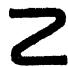
\includegraphics[keepaspectratio]{images/part002_77aeac5d.jpg}}

读者应当警惕，不要以为映射 \((x, y) \to xy\)（一致空间 \(G_{d} \times G_{d}\) 到一致空间 \(G_{d}\) 中的）一般是一致连续的。类似地，对称映射 \(x \to x^{-1}\)（视为 \(G_{d}\) 到 \(G_{d}\) 上的映射时）一般不是一致连续的（见习题 3 与 4）。

命题 3 每个连续同态 \(f\)（拓扑群 \(G\) 到拓扑群 \(G'\) 中的），视为 \(G_d\) 到 \(G_d'\) 中（或 \(G_s\) 到 \(G_s'\) 中）的映射时，是一致连续的。

因为若 \(V'\) 是 \(G'\) 中单位元的一个邻域，且 \(\mathbf{V} = f^{-1}(\mathbf{V}')\)，则关系 \(yx^{-1} \in V\) 蕴含

\[
f (y) (f (x)) ^ {- 1} = f (y x ^ {- 1}) \in V ^ {\prime}.
\]

